\begin{titlepage}
    % Lệnh chèn ảnh nền phủ toàn bộ trang bìa
    \AddToShipoutPictureBG*{
        \AtPageLowerLeft{
            \transparent{1}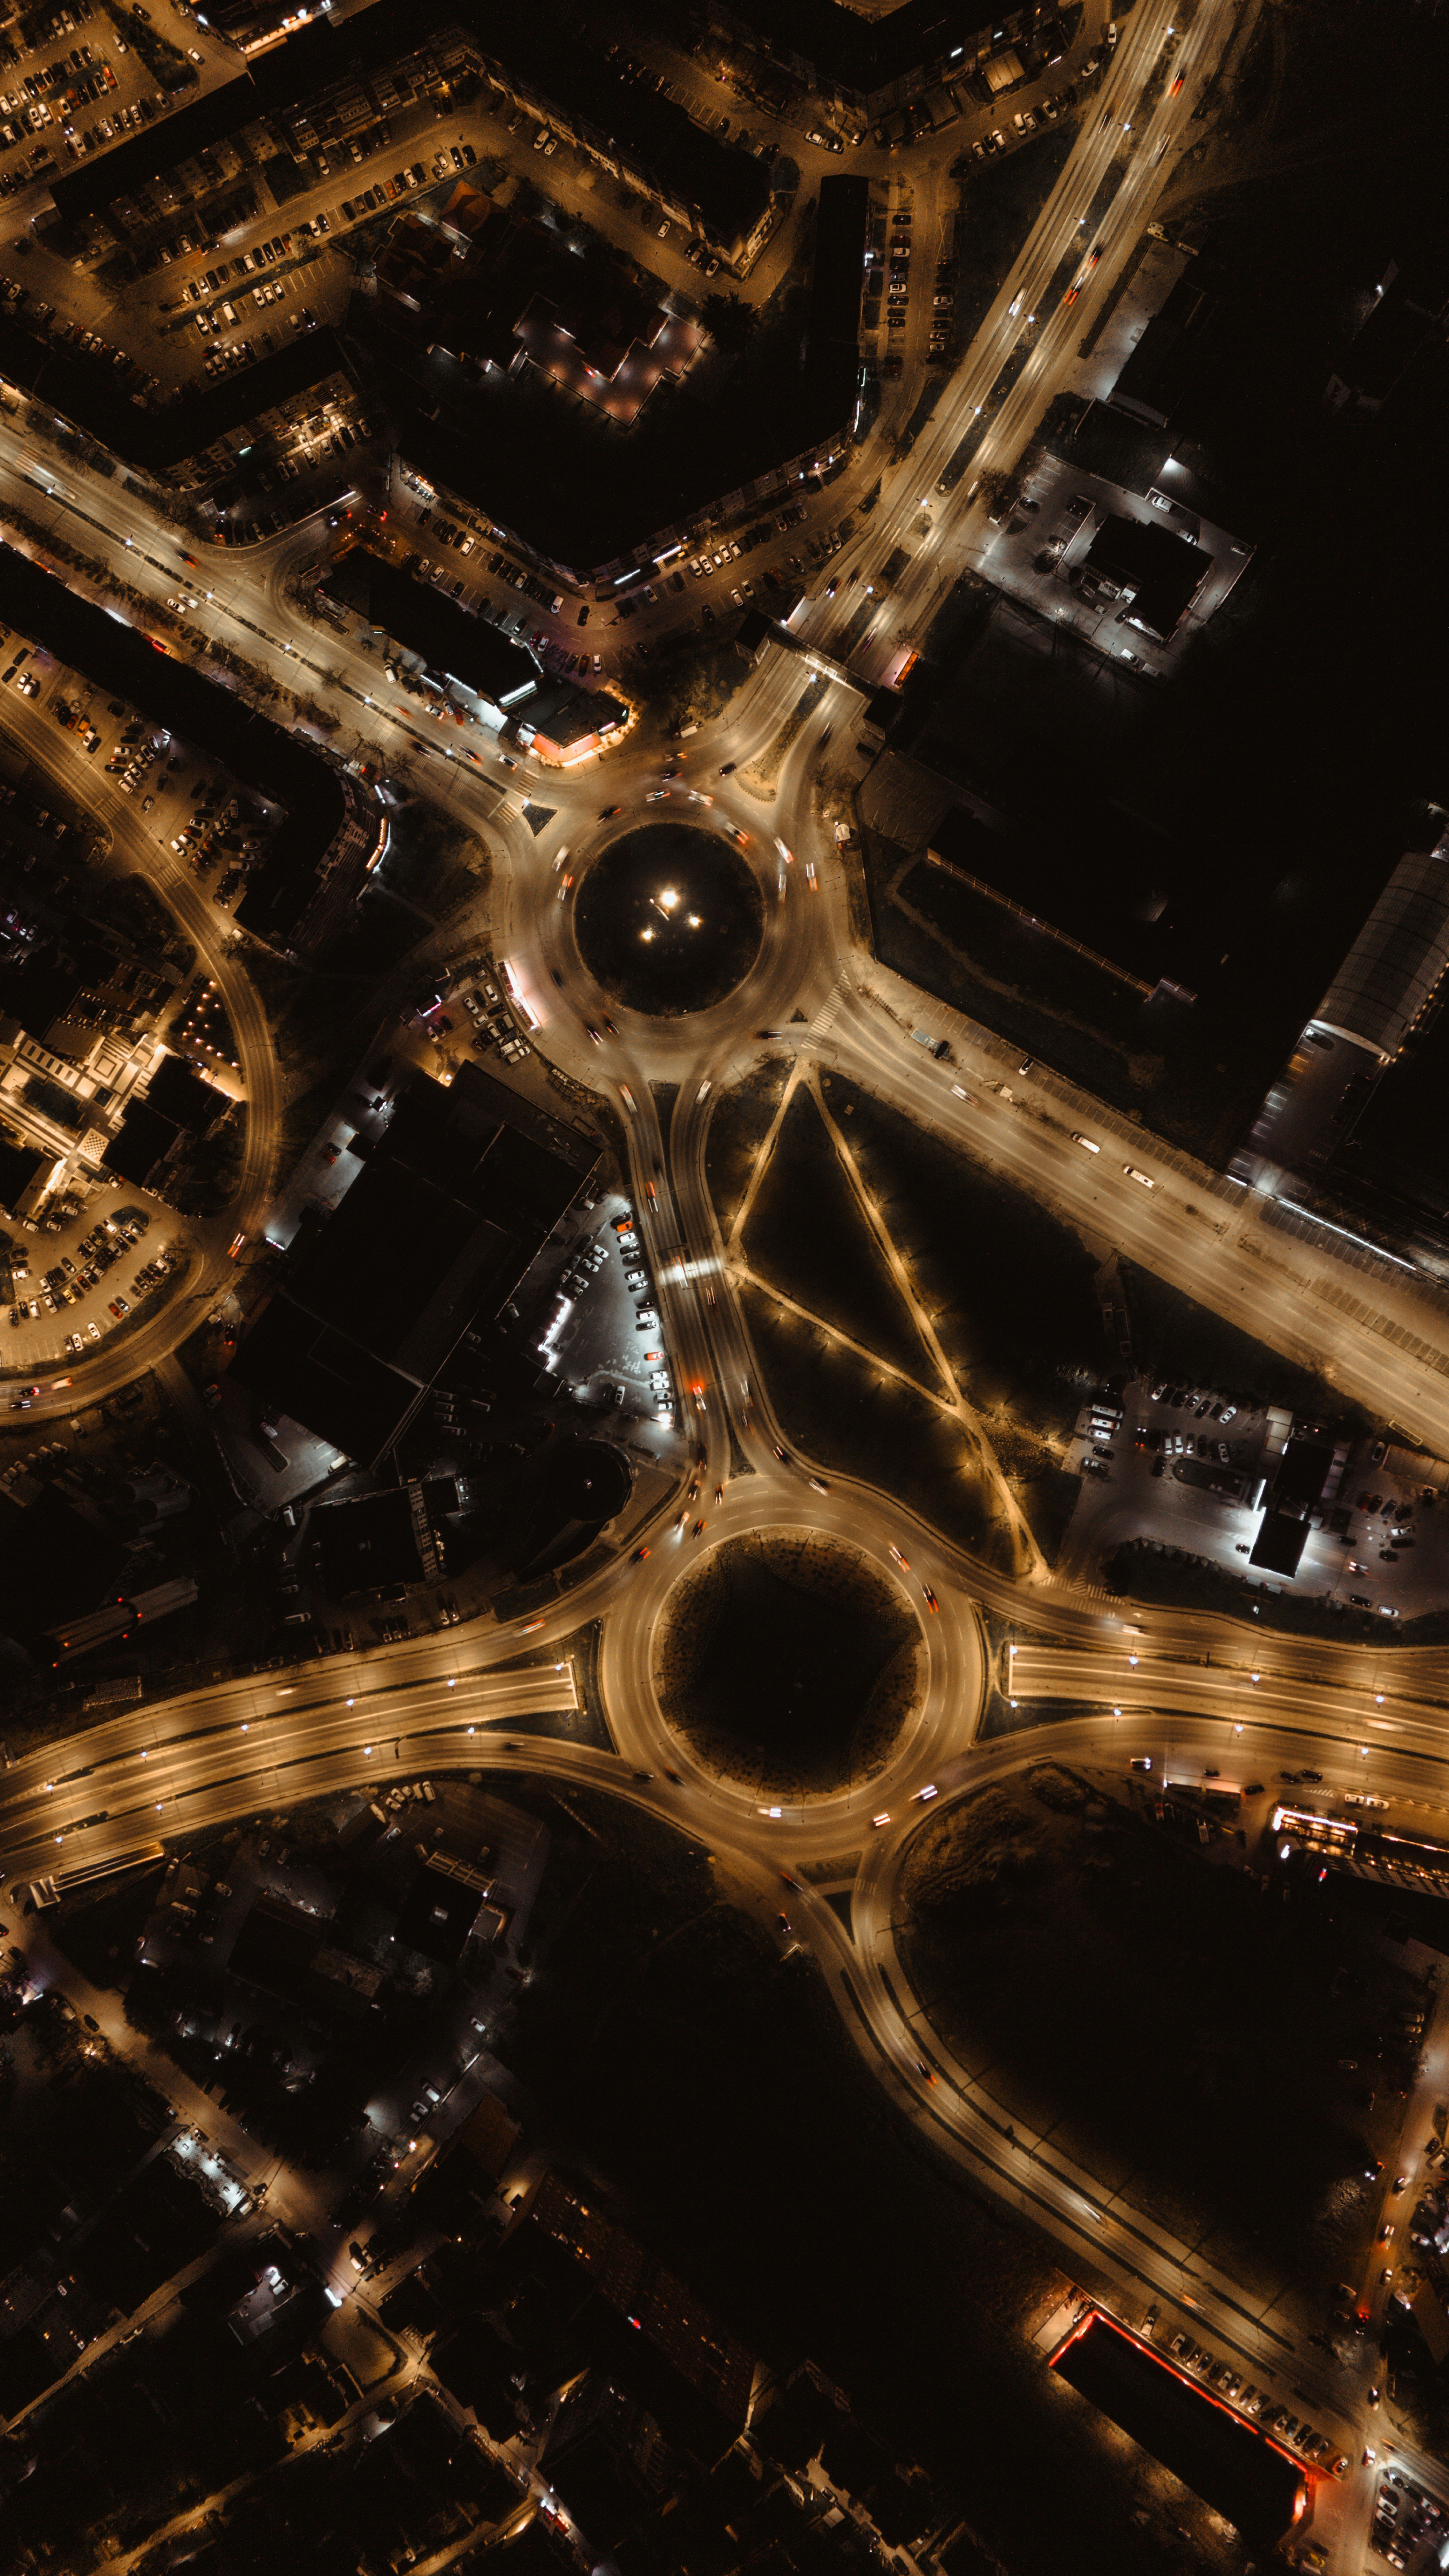
\includegraphics[width=\paperwidth, height=\paperheight]{background2.jpg}
        }
    }
    
    \centering
    \color{white} % Chuyển màu chữ thành màu trắng (hoặc màu tương phản với ảnh nền)
    
    \vspace*{1cm}
    {\large \textbf{BỘ GIÁO DỤC VÀ ĐÀO TẠO}} \\[0.5cm]
    {\large \textbf{TRƯỜNG TRUNG CẤP Y KHOA VIỆT NAM}} \\[3cm]
    
    {\large \textbf{TÀI LIỆU TỔNG HỢP}} \\[0.5cm]
    {\Huge \bfseries KỸ THUẬT THỰC HÀNH \\[0.2cm] VÀ HUYỆT VỊ} \\[4cm]

    \vfill
    
    \begin{flushright}
        \begin{tabular}{ll}
            \textbf{GVHD:} & Trương Văn Chúc \\
            \textbf{SVTH:} & Dương Tiến Mạnh \\
            \textbf{Lớp:} & K12 - Xoa bóp bấm huyệt \\
        \end{tabular}
    \end{flushright}
    
    \vspace{2cm}
    {\large Hà Nội, năm 2026}

\end{titlepage}

% Từ trang sau, ảnh nền sẽ tự động biến mất và màu chữ quay lại mặc định
\newpage 
